
	\documentclass[letter]{article}
	\usepackage{amsmath,amssymb}
	\usepackage[inline]{enumitem}
	\usepackage{blindtext}
	\usepackage{booktabs}
	\usepackage{graphicx}
	\begin{document}
	
	\title{STAT 500 Homework 2}
	\author{Yifan Zhu}
	\maketitle
	
	\begin{enumerate}[leftmargin = 0 em, label = \arabic*., font = \bfseries]

	\item \begin{enumerate}
		\item \textbf{experimental units:} 20 human volunteers

		\textbf{treatments:} drug $A$, drug $B$

		\textbf{response variable:}  white blood cell counts

		\textbf{control:} \begin{enumerate*}[label = (\roman*)]
			\item  specimens to be drawn just before the drug is administered and at 24 hours after the administration of the drug; 
			\item same person to draw blood from each subject;
			\item same lab to determine the white blood cell counts for each specimen.
		\end{enumerate*}

		\textbf{randomization:} 20 human volunteers  randomly divided into two groups

		\textbf{replication:} 10 receiving drug $A$ and 10 receiving drug $B$

		\item \textbf{experimental units:} 30 Xbox machines

		\textbf{treatments:} old fan, two fans, high quality fan

		\textbf{response variable:} time until  machine overheats

		\textbf{control:} \begin{enumerate*}
			\item control group of 10 machines installed the old fan;
			\item  a large room keep at a constant 72 degrees Fahrenheit with 30 different stations setup in equally spaced distances across the room
			\item same style television and television stand
			\item run with the same graphic intensive game
room.
		\end{enumerate*}
		

		\textbf{randomization:} rolling the dice to assign 30 machines to 3 different groups

		\textbf{replication:} 10 machines in each group

		\item \textbf{experimental units:}  60 one-week old soybean seedlings

		\textbf{treatments:} 3 types of plant nutrient ($A$, $B$ or $C$) applied to the soil in the pots for each group

		\textbf{response variable:} dried weight after 10, 20, 30 and 40 days' growth

		\textbf{control:} \begin{enumerate*}[label = (\roman*)]
		\item all one week old
		\item set in individual pot in one green house
		\item drying process 
		\end{enumerate*}

		\textbf{randomization:} \begin{enumerate*}[label = (\roman*)]
		\item 60 pots randomly divided into 3 groups; 
		\item 5 pot randomly selected in each group after evey 10 days' growth.
		\end{enumerate*}

		\textbf{replication:} \begin{enumerate*}[label = (\roman*)]
			\item 20 pots with soil applied nutrient of the same kind in each group;
			\item 5 pots selected in each group every 10 days.
		\end{enumerate*}
		
		

		\item \textbf{experimental units:} 20 specimens

		\textbf{treatments:} standard method, new method

		\textbf{response variable:} concentration of the solution

		\textbf{control:}\begin{enumerate*}[label = (\roman*)]
			\item 20 specimens from the same batch of solution with a specific concentration of compound;
			\item same person to analyze all specimens;
		\end{enumerate*}
		

		\textbf{randomization:} 10 specimens randomly assigned to be analyzed with standard method and the other 10 with new method

		\textbf{replication:} 10 specimens analyzed with the same method

		\item \textbf{experimental units:} 1,200 soybean plants

		\textbf{treatments:} usual pesticide, new organic pesticide, untreated

		\textbf{response variable:}  proportion of infected soybean plants in each plot

		\textbf{control:}  \begin{enumerate*}[label = (\roman*)]
			\item land far from any  trees to prevent any area getting less sunlight to plant soybeans;
			\item each plot watered equally by the same farmer and using the same equipment
		\end{enumerate*}
		

		\textbf{randomization:}  randomly choosing 10 plots to receive usual pesticide, 10 plots to receive a new organic pesticide, and the last 10 plots were left untreated

		\textbf{replication:} 10 plots to get the same treatments and 40 soybean plants in each plot

		

		
	\end{enumerate}
\newpage
	\item 
	Denote the sample mean of survival times with Bacilli treatment $\overline{Y_1}$, sample mean of survail times in the control group $\overline{Y_2}$, expectation of  of survival time with Bacilli treatment $\mu_1$, expectation of survail time in the control group $\mu_2$.

	$H_0:\, \mu_1 - \mu_2 = 0$

	$H_a:\, \mu_1 - \mu_2 \neq 0$

	test statistic: $\overline{Y_1} - \overline{Y_2}$

	oberved test statistics: $\overline{Y_1} - \overline{Y_2} = 102.69$

	p-value: 0.28\%

	decision: reject $H_0$

	conclusion: there is difference in survival times between two treatments

\begin{table}[!htb]
\caption{Differences as Extreme as the Observed Difference (102.69)}
	\begin{tabular}{ccccccccc}
	\toprule
	Obs & sample & n1 & mean1 & css1 & n2 & mean2 & css2 & diff\\ 
	\midrule
1&3252&58&227.552&1320272.34&64&358.797&2380060.36&-131.245\\
2&4795&58&231.362&1570027.40&64&355.344&2186710.44&-123.982\\
3&2786&58&232.621&1282443.66&64&354.203&2492220.36&-121.582\\
4&3870&58&234.052&1354166.84&64&352.906&2440453.44&-118.855\\
5&3459&58&234.483&1116184.48&64&352.516&2684357.98&-118.033\\
6&8926&58&236.569&1371854.22&64&350.625&2456771.00&-114.056\\
7&8358&58&239.776&1520548.09&64&347.719&2349368.94&-107.943\\
8&4167&58&239.845&1176373.60&64&347.656&2694406.44&-107.811\\
9&6222&58&240.517&1440398.48&64&347.047&2438740.86&-106.530\\
10&8545&58&240.793&1141899.52&64&346.797&2740640.36&-106.004\\
11&1370&58&241.914&1343452.57&64&345.781&2552728.94&-103.867\\
12&4784&58&242.276&1498929.59&64&345.453&2401599.86&-103.177\\
13&3223&58&242.310&1439354.41&64&345.422&2461587.61&-103.112\\
14&4721&58&242.483&1496336.48&64&345.266&2406664.48&-102.783\\
15&9271&58&350.483&2164246.48&64&247.391&1736817.23&103.092\\
16&2589&58&350.759&2451534.62&64&247.141&1446221.73&103.618\\
17&7438&58&350.914&2311334.57&64&247.000&1584554.00&103.914\\
18&7246&58&351.776&2360392.09&64&246.219&1525022.94&105.557\\
19&8036&58&352.672&2275648.78&64&245.406&1598699.44&107.266\\
20&1462&58&353.000&2184956.00&64&245.109&1685304.23&107.891\\
21&4996&58&354.138&2187582.90&64&244.078&1668292.61&110.060\\
22&8413&58&354.414&2274582.07&64&243.828&1577763.11&110.586\\
23&9994&58&354.897&2301007.38&64&243.391&1545119.23&111.506\\
24&6390&58&355.845&2214001.60&64&242.531&1619759.94&113.314\\
25&3204&58&356.034&2349153.93&64&242.359&1482110.73&113.675\\
26&8504&58&357.328&2403198.78&64&241.188&1410829.75&116.140\\
27&1243&58&358.069&2270599.72&64&240.516&1533379.98&117.553\\
28&8262&58&367.741&2522509.12&64&231.750&1139232.00&135.991\\
\bottomrule
	\end{tabular}
	\end{table}

	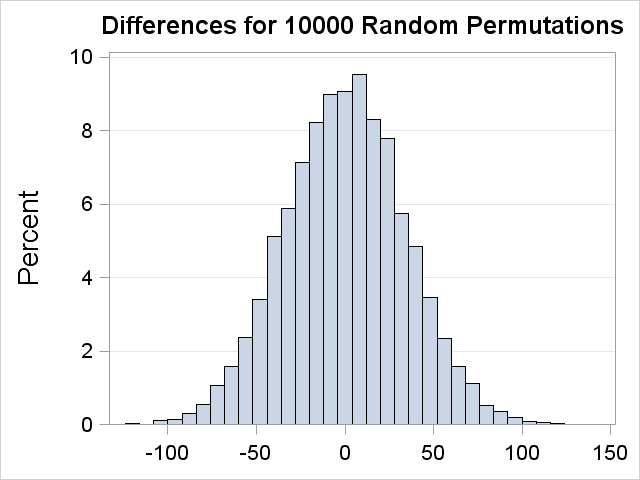
\includegraphics[width = \textwidth]{guinea_random_permutation.png}
	
	
 	\end{enumerate}


	
	
	
	\end{document}